\documentclass{article}
\usepackage{tikz}
\usetikzlibrary{arrows.meta, positioning, shapes.geometric}

\begin{document}

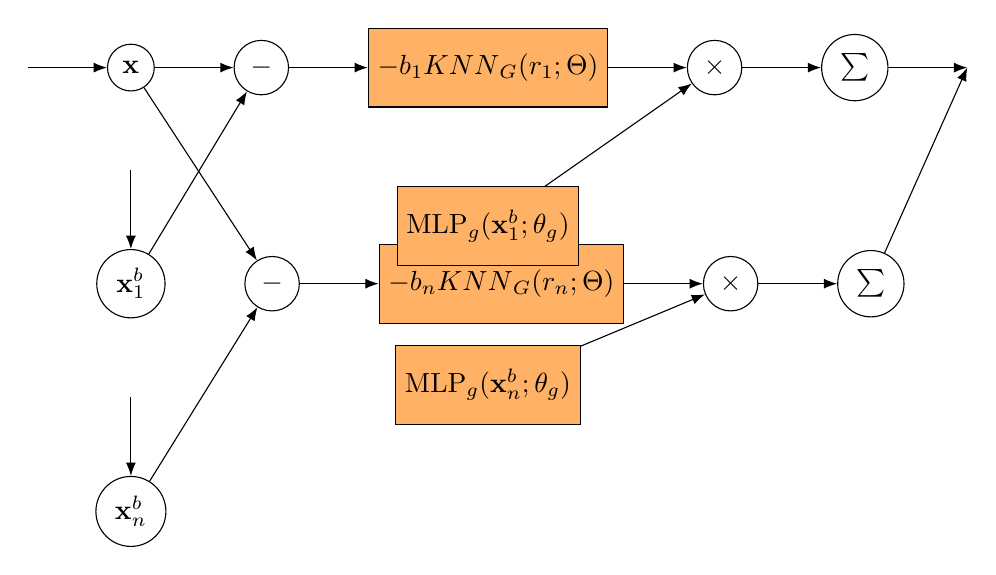
\begin{tikzpicture}[node distance=1cm, auto,
    neuron/.style={circle, draw, minimum size=0.5cm},
    activation/.style={rectangle, draw, fill=orange!60, minimum width=2cm, minimum height=1cm},
    sum/.style={circle, draw, minimum size=0.5cm},
    multiply/.style={circle, draw, minimum size=0.5cm},
    input/.style={coordinate},
    output/.style={coordinate},
]

% Input nodes
\node[input] (input) {};
\node[neuron, right=of input] (x) {$\mathbf{x}$};
\node[input, below=of x] (input2) {};
\node[neuron, below=of input2] (x1) {$\mathbf{x}_1^b$};
\node[input, below=of x1] (input3) {};
\node[neuron, below=of input3] (xn) {$\mathbf{x}_n^b$};

% Distance nodes
\node[neuron, right=of x] (r1) {$-$};
\node[neuron, right=of x1] (rn) {$-$};

% KNN nodes
\node[activation, right=of r1] (knn1) {$-b_1 \text{KNN}_{G}(r_1; \Theta)$};
\node[activation, right=of rn] (knnn) {$-b_n \text{KNN}_{G}(r_n; \Theta)$};

% Multiply nodes
\node[multiply, right=of knn1] (mul1) {$\times$};
\node[multiply, right=of knnn] (muln) {$\times$};

% Sum node
\node[sum, right=of mul1] (sum1) {$\sum$};
\node[sum, right=of muln] (sumn) {$\sum$};

% Output node
\node[output, right=of sum1] (output) {$u(\mathbf{x})$};

% MLP nodes
\node[activation, below=of knn1] (mlp1) {MLP$_g(\mathbf{x}_1^b; \theta_g)$};
\node[activation, below=of mlp1] (mlpn) {MLP$_g(\mathbf{x}_n^b; \theta_g)$};

% Arrows
\draw[-Latex] (input) -- (x);
\draw[-Latex] (x) -- (r1);
\draw[-Latex] (x) -- (rn);
\draw[-Latex] (input2) -- (x1);
\draw[-Latex] (x1) -- (r1);
\draw[-Latex] (input3) -- (xn);
\draw[-Latex] (xn) -- (rn);

\draw[-Latex] (r1) -- (knn1);
\draw[-Latex] (rn) -- (knnn);

\draw[-Latex] (knn1) -- (mul1);
\draw[-Latex] (knnn) -- (muln);

\draw[-Latex] (mul1) -- (sum1);
\draw[-Latex] (muln) -- (sumn);

\draw[-Latex] (mlp1) -- (mul1);
\draw[-Latex] (mlpn) -- (muln);

\draw[-Latex] (sum1) -- (output);
\draw[-Latex] (sumn) -- (output);

\end{tikzpicture}

\end{document}